\subsection{Bestehende Konzepte und zukünftige Flugzeugmodelle}
In diesem Teil ist beschrieben, welche Flugzeugmodelle und -konfigurationen 
mit im Teil \ref{s:Neuartige Antriebe} beschriebenen Antrieben in näherer Zukunft zu erwarten sind. 
Vor allem sind hier die Modelle ohne hybride Nutzung fossiler Energieträger zusammengefasst.

Aufgrund ihrer Drop-In Fähigkeit werden die SAFs keine neuen Luftfahrzeugkonfigurationen brauchen. 
Was als Vorteil für den SAF betrachtet werden kann, angesichts der aktuell produzierten Flugzeuge, 
die mindestens 20 Jahr im Einsatz sein werden (Quelle).
Die Abbildung stellt Eintrittsjahre für alternative Antriebe dar.
Kleinere Flugzeuge mit sowohl elektrischem Antrieb, als auch der Brennstoffzelle sind bereits jetzt im Einsatz zu finden.
%
\begin{figure}[h]
	\centering
	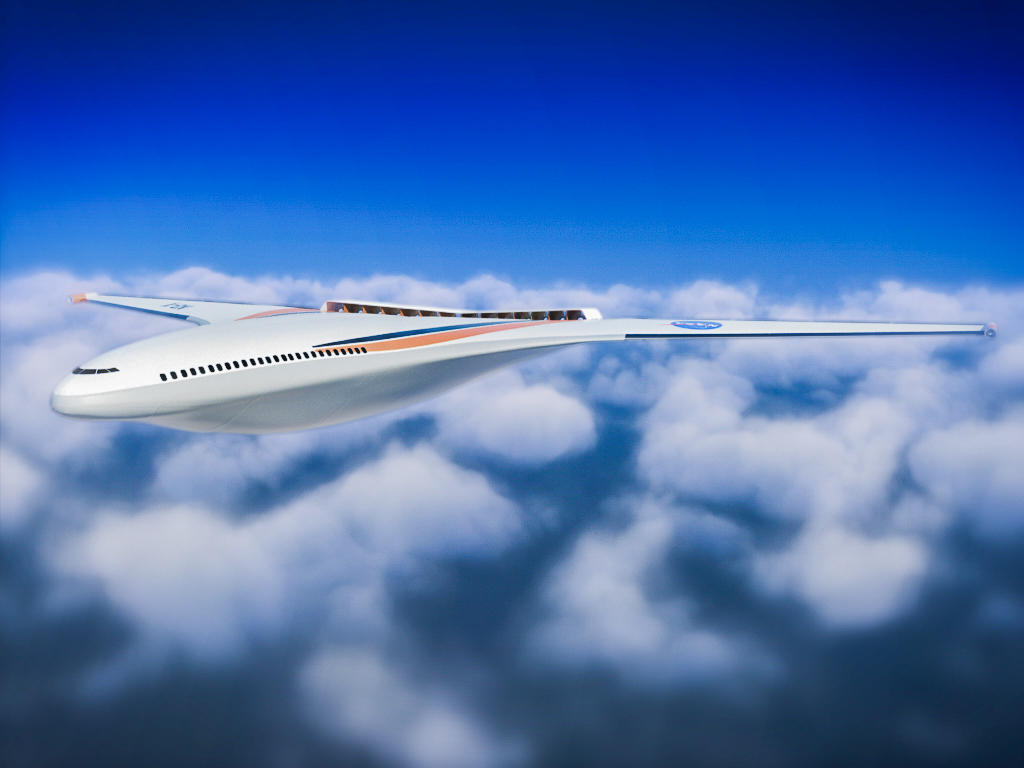
\includegraphics[width=0.6\linewidth]{Bilder/NASA.jpg}
	\caption[NASA]{NASA}
	\label{NASA_konfig}
\end{figure}
%
Positive Auswirkungen auf die Emissions-Werte können bereits mit bestimmten 
Flugzeug- und Triebwerkskonfigurationen erreicht werden.
Zum Beispiel \textit{Claire Liner} vom Bauhaus Luftfahrt e. V. München 
bringt nicht nur aerodynamische Vorteile mit, sondern auch eine Verringerung 
des Kraftstoffverbrauchs und damit die Reduktion der Emissionen.
Jedoch sind mehr Änderungen notwendig, um Netto null \ce{CO2}-Werte zu erreichen.
Die Herstellung bereitet Schwierigkeiten, manche Firmen müssen den Geschäftsbetrieb einstellen, 
wie Universal Hydrogen oder Zunum Aero, oder Konzepte werden nicht weiterentwickelt.

Es wurden eine Vielzahl an elektrischen Flugzeugen mit geringer 
Sitzkapazität vorgestellt, einige davon wurden sogar geflogen.
Das Institut für Flugzeugbau der Universität Stuttgart entwickelte 
ein zweisitziges hybrid-batteriebetriebenes Segelflugzeug \textit{e-Genius}. 
Das Flugzeug soll eine Reichweite von 400 km erreichen und hat eine 
Batteriekapazität von 40 kWh mit 1,5 Stunden Ladedauer. %Quelle https://www.ifb.uni-stuttgart.de/en/research/mannedaircraft/e-genius/
Pipistrel Alpha Electro hat bereits im Jahr 2007 sein ersten elektrischen Zweisitzer vorgestellt, 
mittlerweile wird das Modell "Velis Electro" \cite{Pipistrel_VelisElectro} für 
das Pilottraining mit einem Triebwerk mit 57.6 kW Leistung genutzt. 
Der Antrieb ist flüssigkeitsgekühlt und braucht ein externes Ladegerät.
Die größeren Konzepte hingegen haben aufgrund der Komplexität der Technologien 
und Gewicht mit der Umsetzung zu kämpfen.\\


\paragraph{Konfigurationen mit Batterie-Antrieb}
Wie bereits erwähnt wurde, haben die zurzeit bestehenden Batterien die geringe Energiedichte. 
Deshalb ist zu erwarten, dass bis zum Jahr 2050 keine großen vollelektrischen Flugzeuge hergestellt werden, 
stattdessen werden die Regional- und Kurzstrecken in den Mittelpunkt gestellt.

Ein vielversprechender Prototyp war die \textit{ES-19} von Heart Aerospace. 
Das Unternehmen versprach die Beförderung von 19 Passagieren über 400 km mit einem BA. 
Das Flugzeug war für die Regionalstrecken konzipiert und 
somit konnte die geringe Nachfrage gedeckt werden. 
Außerdem wurden geringe Betriebs- und Wartungskosten erwartet (Quelle).
Das aktuellste Modell ES-30 wurde jedoch auf einen hybriden Antrieb umgerüstet.

Eines der größten Konzepte mit vollelektrischen Abtrieb stellte Bauhaus Luftfahrt vor. 
Das Passagierflugzeug \textit{Ce-Liner} \cite{BauhausLuftfahrt} ist mit einer C-Wing-Konfiguration
ausgestattet und sollte eine Reichweite von 900 NM haben und 190 Passagiere befördern. 
Die benötigte Batteriekapazität wurde auf 2000 Wh/kg eingeschätzt. 
Die Batteriemodule sollen bei Turnaround ausgewechselt werden.


\textbf{Konfigurationen mit Wasserstoff-Antrieb}

Embraer zeigte eine Reihe von nachhaltigen Flugzeugen \textit{ENERGIA}. 
Die Flugzeuge sind mit unterschiedlichen Antrieben ausgestattet, 
unter anderem hybrid-elektrisch oder mit Wasserbrennstoffzelle und Wasserstoffturbine. 
Bei der Wasserstoffturbine wurde das Konzept von Dualem-Treibstoff vorgeschlagen, 
bei welchem entweder Jet-A/SAF oder Wasserstoff genutzt werden kann. 
Das Unternehmen spricht von einer Technologiebereitschaft ab dem Jahr 2030, 
für die Wasserstoffturbine ab dem Jahr 2035 und der Wasserstoffturbine ab dem Jahr 2040. \cite{embraer_energia_2021}
%
Airbus \cite{airbus_zea_concepts} hat im Jahr 2020 drei unterschiedliche 
emissionsfreie \textit{ZEROe} Konzepte vorgestellt: Turbofan, Turboprop und eins mit „Blended-wing body“-Design.
In allen Konzepten ist Wasserstoff im Einsatz und Antrieb mit Gasturbinentriebwerk. 
Die Reichweite bewegt sich in einem Bereich von über 1.850 - 3700 km 
und die Anzahl beförderter Passagiere wird von auf 100 bis 200 geschätzt. 
Das Unternehmen will die Technologien bis zum 2035 zur Einsatzreife bringen.

Wright Spirit \cite{wright_electric_website} hat ein Konzept auf Basis 
des konventionellen Flugzeugs BAe 146 vorgestellt, allerdings mit einem Wasserstoff-Antrieb.
Das Flugzeug soll mit 4 Triebwerken, 2,5 MW Motoren und vorgestellter Batterie 
mit 800 Wh/kg eine Reichweite von 1000 km erreichen und 100 Passagiere transportieren.

NASA hat das turboelektrische, mit flüssigen Wasserstoff angetriebene 
Konzept N3-X \cite{NASA_N3X_2025} vorgeschlagen.
Das Modell ist \textit{hybrid wing body} konzipiert und verspricht, 
dass der Treibstoffverbrauch bis um 70 \% reduziert werden kann.
Universal Hydrogen % MAX: was ist hier?

ZeroAvia stellt ihre hybrid Wasserstoff-elektrischen Antriebe 
mit 3 unterschiedlichen Leistungen und Kapazitäten vor. 
Der kleinste Antrieb, ZA600, hat mit einer Leistung von 600 kW, 
die Möglichkeit bis zu 20 Passagiere über 555 km zu befördern. 
Die Geplante Eintrittzeit (Entry-in-System EIS) ist im Jahr 2025. 
Der Antrieb ist mit gasförmigem Wasserstoff angetrieben.
%Flugzeug mit 80 Menschen verbraucht bis zu 80% weniger Treibstoff pro STD/kg (5 mal weniger)




Aufgrund des schweren und massiven Wasserstofftanks werden 
unterschiedliche wasserstoffkonfugurationen vorgeschlagen.
Es gibt Konzepte, wo der Tank am Rumpf, am Ende des Rumpfes 
oder vorne, hinter der Pilotenkabine sitzt. % MAX: was ist hier?
Abschließend ist zu beobachten, dass aktuell viele Konzepte ausgearbeitet werden. 
Wie erfolgreich diese sind, ist abzuwarten bis Technologien tatsächlich auf den Markt kommen.
